\documentclass[11pt]{article}
\usepackage[utf8]{inputenc}
\usepackage[a4paper]{geometry}
\usepackage{amsmath}
\usepackage{amssymb}
\usepackage{amsthm}
\usepackage{array}
\usepackage{chngcntr}
\usepackage{commath}
\usepackage{comment}
\usepackage{enumitem}
\usepackage{hyperref}
\usepackage{stmaryrd}
\usepackage{thmtools}
\usepackage{tikz}
\usepackage{tikz-cd}
\usepackage{titlesec}

\theoremstyle{definition}
\newtheorem{definition}{Definition}[section]
\newtheorem*{definition*}{Definition}
\newtheorem*{example}{Example}
\newtheorem*{exercise}{Exercise}
\newtheorem*{fact}{Fact}

\theoremstyle{plain}
\newtheorem{theorem}[definition]{Theorem}
\newtheorem{proposition}[definition]{Proposition}
\newtheorem{lemma}[definition]{Lemma}
\newtheorem{corollary}[definition]{Corollary}

\theoremstyle{remark}
\newtheorem*{remark}{Remark}

\renewcommand{\qedsymbol}{$\blacksquare$}

\DeclareMathOperator{\Char}{char}
\DeclareMathOperator{\Gal}{Gal}
\DeclareMathOperator{\id}{id}
\DeclareMathOperator{\area}{area}

\newcommand{\FF}{\mathbb{F}}
\newcommand{\NN}{\mathbb{N}}
\newcommand{\ZZ}{\mathbb{Z}}
\newcommand{\QQ}{\mathbb{Q}}
\newcommand{\RR}{\mathbb{R}}
\newcommand{\CC}{\mathbb{C}}
\newcommand{\PP}{\mathbb{P}}
\newcommand{\cD}{\mathcal{D}}
\newcommand{\cO}{\mathcal{O}}
\newcommand{\cP}{\mathcal{P}}
\newcommand{\fp}{\mathfrak{p}}
\newcommand{\fq}{\mathfrak{q}}
\newcommand{\fm}{\mathfrak{m}}

\setlist[enumerate,1]{label=(\roman*), nosep}
\setlist[itemize,1]{nosep}

% Uncomment to exclude proofs
% \excludecomment{proof}

\title{Part III Elliptic Curves Lecture Notes}
\author{Ming Yean Lim}

\begin{document}

\maketitle

\noindent These lecture notes were based on the Part III course Elliptic Curves taught during Lent 2023 by Professor Tom Fisher.

% \tableofcontents

% \newcommand{\sectionbreak}{\clearpage}

\section{Fermat's Method of Infinite Descent}

Let $\Delta$ be the right-angled triangle
\begin{center}
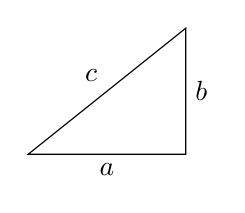
\begin{tikzpicture}[scale=1, transform shape]
    \draw (0,0) -- node[auto, swap]{$a$} (2,0) -- node[auto, swap]{$b$} (2,1.6) -- node[auto, swap]{$c$} cycle;
\end{tikzpicture}
\end{center}
We have $a^2 + b^2 = c^2$, and $\area(\Delta) = \frac{1}{2} a b$.

\begin{definition*}
    We say $\Delta$ is \emph{rational} if $a, b, c \in \QQ$, and $\Delta$ is \emph{primitive} if $a, b, c \in \ZZ$ are coprime\footnote{this is equivalent to $a, b, c$ being pairwise coprime}.
\end{definition*}

\begin{lemma}\label{lem:1_1}
    Every primitive triangle\footnote{we allow swapping edges $a$ and $b$} is of the form
    \begin{center}
    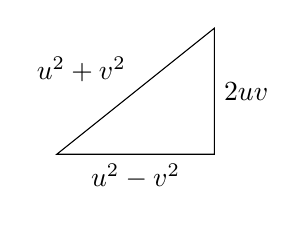
\begin{tikzpicture}[scale=1, transform shape]
        \draw (0,0) -- node[auto, swap]{$u^2 - v^2$} (2,0) -- node[auto, swap]{$2uv$} (2,1.6) -- node[auto, swap]{$u^2 + v^2$} cycle;
    \end{tikzpicture}
    \end{center}
    for some integers $u > v > 0$.
\end{lemma}
\begin{proof}
    $a$ and $b$ cannot be both odd, otherwise $c \equiv 2 \pmod{4}$, which has no solutions. They cannot be both even either, since we are assuming the triangle to be primitive.

    WLOG $a$ is odd and $b$ is even, so that $c$ is odd. Then
    \begin{equation*}
        \left(\frac{b}{2}\right)^2 = \frac{c+a}{2} \frac{c-a}{2}
    \end{equation*}
    is a product of coprime positive integers. Indeed $(\frac{c+a}{2}, \frac{c-a}{2}) \mid (a, c) = 1$. Thus by unique factorisation in $\ZZ$, $\frac{c+a}{2} = u^2$ and $\frac{c-a}{2} = v^2$ for some $u, v \in \ZZ$. Then $a = u^2 - v^2$, $b = 2uv$, and $c = u^2 + v^2$.
\end{proof}

\begin{definition*}
    $D \in \QQ_{> 0}$ is a \emph{congruent number} if there exists a rational right-angled triangle with $\area(\Delta) = D$.
\end{definition*}

\noindent To find all congruent numbers, it suffices to consider $D \in \ZZ_{>0}$ squarefree.

\begin{example}
    $D = 5, 6$ are congruent numbers.
\end{example}

\begin{lemma}\label{lem:1_2}
    $D \in \QQ_{> 0}$ is a congruent number if and only if $D y^2 = x^3 - x$ for some $x, y \in \QQ$ with $y \neq 0$.
\end{lemma}
\begin{proof}
    \autoref{lem:1_1} shows that $D$ is congruent iff $D w^2 = u v (u^2 - v^2)$ for some $u, v, w \in \QQ$ with $w \neq 0$. Setting $x =\frac{u}{v}$ and $y = \frac{w}{v^2}$ gives the equation in the lemma.
\end{proof}

\begin{theorem}\label{thm:1_3}
    There is no solution to
    \begin{equation}\label{eqn:1_3_star}
        w^2 = u v (u + v) (u - v) \quad \text{ for } u, v, w \in \ZZ, w \neq 0
    \end{equation}
\end{theorem}
\begin{proof}
    Suppose we have a solution $u, v, w$. Dividing out the common factor of $u$ and $v$, we may assume that $u, v$ are coprime. By flipping signs of $u, v$, we may assume that $u > 0$. Clearly we can assume $w > 0$. We can also assume $v > 0$: if $v < 0$, then replace $(u, v, w)$ by $(-v, u, w)$. If $u \equiv v \pmod{2}$, then replace $(u, v, w)$ by $(\frac{u+v}{2}, \frac{u-v}{2}, \frac{w}{2})$.

    Thus $u, v, u+v, u-v$ are pairwise coprime\footnote{$(u+v, u-v) \mid 2(u, v) = 2$, but $u \pm v$ are both odd, so $(u+v, u-v) = 1$} positive integers with their product a square. By unique factorisation in $\ZZ$, $u = a^2$, $v = b^2$, $u+v = c^2$, and $u-v = d^2$ for some $a, b, c, d \in \ZZ$. Since $u \not\equiv v \pmod{2}$, $c, d$ are both odd. Then
    \begin{equation*}
        \left(\frac{c+d}{2}\right)^2 + \left(\frac{c-d}{2}\right)^2 = \frac{c^2 + d^2}{2} = u = a^2
    \end{equation*}
    Then
    \begin{center}
    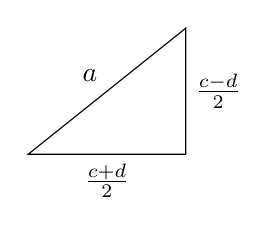
\begin{tikzpicture}[scale=1, transform shape]
        \draw (0,0) -- node[auto, swap]{$\frac{c+d}{2}$} (2,0) -- node[auto, swap]{$\frac{c-d}{2}$} (2,1.6) -- node[auto, swap]{$a$} cycle;
    \end{tikzpicture}
    \end{center}
    is a primitive triangle of area $\frac{c^2 - d^2}{8} = \frac{v}{4} = (\frac{b}{2})^2$. Let $w_1 = \frac{b}{2}$. Let $u_1, v_1 \in \ZZ$ be the $u, v$ in \autoref{lem:1_1} corresponding to this triangle. Then $w_1^2 = u_1 v_1 (u_1 + v_1) (u_1 - v_1)$, which gives a new solution to \eqref{eqn:1_3_star}. We have $4 w_1^2 = b^2 = v \mid w^2$ implies $w_1 \le \frac{w}{2}$, so we have a solution with a smaller $w$. By Fermat's method of infinite descent, there is no solution to \eqref{eqn:1_3_star}.
\end{proof}

Now we will see a variant of this for polynomials. In this section , we let $K$ be a field with $\Char K \neq 2$, and $\overline{K}$ its algebraic closure.

\begin{lemma}\label{lem:1_4}
    Let $u, v \in K[t]$ be coprime. If $\alpha u + \beta v$ is a square for 4 distinct $(\alpha : \beta) \in \PP^1$, then $u, v \in K$.
\end{lemma}
\begin{proof}
    WLOG $K = \overline{K}$ is algebraically closed. By changing coordinates\footnote{$u, v$ are replaced by an invertible linear combination} on $\PP^1$, we may assume that the ratios $(\alpha : \beta)$ are $(1 : 0), (0 : 1), (1 : -1), (1 : -\lambda)$ for some $\lambda \in K \setminus \{0,1\}$.
    \begin{align*}
        u &= a^2\\
        v &= b^2\\
        u-v &= (a+b)(a-b)\\
        u-\lambda v &= (a+\mu b)(a-\mu b)
    \end{align*}
    for some $a, b \in K[t]$, and $\mu = \sqrt{\lambda}$. By unique factorisation in $K[t]$, $a+b, a-b, a+\mu b, a-\mu b$ are squares. But\footnote{$\max\{\deg{u}, \deg{v}\}$ does not change when we replace $u, v$ with an invertible linear combination} $\max\{\deg{a}, \deg{b}\} \le \frac{1}{2} \max\{\deg{u}, \deg{v}\}$, so by Fermat's method of infinite descent, $u, v \in K$.
\end{proof}

\begin{definition}\label{def:1_5}\phantom{}
    \begin{enumerate}
        \item An \emph{elliptic curve} $E/K$ is the projective closure of the plane affine curve
            \begin{equation}\label{eqn:weierstrass_eqn}
                Y^2 = f(X)
            \end{equation}
            where $f \in K[X]$ is a monic cubic polynomial with distinct roots in $\overline{K}$. \eqref{eqn:weierstrass_eqn} is called a Weierstrass equation.

        \item For $L/K$ a field extension, set $E(L) = \{(x, y) \in L \mid y^2 = f(x)\} \cup \{0\}$, where $0$ denotes the point at infinity.
    \end{enumerate}
\end{definition}

\begin{fact}
    $E(L)$ is naturally an abelian group.
\end{fact}

In this course we will study $E(K)$ for $K$ a finite field, local field ($[K : \QQ_p] < \infty$), and number field.

\autoref{lem:1_2} and \autoref{thm:1_3} imply that for $E : Y^2 = X^3 - X$, we have $E(\QQ) = \{0, (0, 0), (\pm 1, 0)\}$. As we will see, this is a group isomorphic to $C_2 \times C_2$.

\end{document}
